\documentclass[a4paper, 12pt]{article}%тип документа

%отступы
\usepackage[left=2cm,right=2cm,top=2cm,bottom=3cm,bindingoffset=0cm]{geometry}
\setlength{\parindent}{5ex}

%Русский язык
\usepackage[T2A]{fontenc} %кодировка
\usepackage[utf8]{inputenc} %кодировка исходного кода
\usepackage[english,russian]{babel} %локализация и переносы

%Вставка картинок
\usepackage{graphicx}
\graphicspath{{pictures/}}
\DeclareGraphicsExtensions{.pdf,.png,.jpg}

%Графики
\usepackage{pgfplots}
\pgfplotsset{compat=1.9}

%Математика
\usepackage{amsmath, amsfonts, amssymb, amsthm, mathtools}

%Таблицы
\usepackage{longtable} 
\usepackage{float}

%Римские цифры
\newcommand{\RomanNumeralCaps}[1]{\uppercase\expandafter{\romannumeral#1}}

\usepackage{multirow}

\usepackage{hhline}

\begin{document}
	\begin{titlepage}
		\begin{center}
			\textsc{Федеральное государственное автономное образовательное учреждение высшего образования«Московский физико-технический институт (национальный исследовательский университет)»\\[5mm]
			}
			
			\vfill
			
			\textbf{Вопрос по выбору: \\[3mm]
				Интерферометр Жамена.
				\\[50mm]
			}
			
		\end{center}
		
		\hfill
		\begin{minipage}{.5\textwidth}
			Выполнили студенты:\\[2mm]
			Сериков Василий Романович\\[2mm]
			Группа: Б03-102\\[5mm]
			Сериков Алексей Романович\\[2mm]
			Группа: Б03-103\\[5mm]
			
		\end{minipage}
		\vfill
		\begin{center}
			Москва, 2023 г.
		\end{center}
		
	\end{titlepage}
	
	\newpage
	\textbf{Аннотация}\\
	
	
	\textbf{Цель работы: }\\
	
	Измерение показателей преломления газов с помощью интерферометра Жамена.\\
	
	\textbf{В работе используется: }\\
	
	Интерферометр Жамена, газовая кювета,
	осветитель, зрительная труба, сильфон, баллон с углекислым газом,
	манометр, краны.\\
	
	\textbf{Теория: }\\
	
	Главной частью интерферометра Жамена являются две одинаковые толстые плоскопараллельные стеклянные
	пластинки $P_1$ и $P_2$, посеребрённые с одной стороны. расположены они так, чтобы между их плоскостями был небольшой угол.
	
	\begin{figure}[H]
		\center{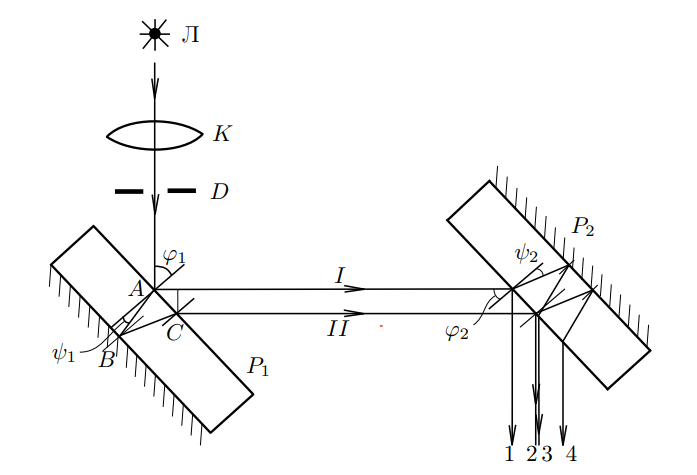
\includegraphics[scale=0.6]{ust.png}}
		\caption{Ход лучей в интерферометре Жамена}
	\end{figure}
	
	На выходе интерферометра оказывается 4 луча. Наименьшая разность хода только между лучами 2 и 3. Между остальными, в силу большой толщины пластинок, большая разность хода. Поэтому интерференция возникает только при суперпозиции лучей 2 и 3. Присутствие лучей 1 и 4 ухудшает чёткость интерференционной картины, и поэтому их устраняют с помощью диафрагм.
	
	Подсчитаем разность хода между лучами 2 и 3. Разность хода между лучами I и II, отражёнными от передней и задней поверхности пластинки $P_1$, равна
	\begin{equation}
	\Delta_1 = n(AB + BC) - AH = 2hn \cos \psi_1.
	\end{equation}
	где n — показатель преломления, h — толщина пластинки, $\psi_1$ - угол преломления в пластинке $P_1$. После отражения от поверхностей пластинки
	$P_2$ лучи 2 и 3 приобретают дополнительную разность хода, равную
	\begin{equation}
	\Delta_2 = 2hn\cos \psi_2.
	\end{equation} 
	где $\psi_2$ — угол преломления в пластинке $P_2$. Полная разность хода между
	лучами 2 и 3 равна
	\begin{equation}
	\Delta = \Delta_1 + \Delta_2 = 2hn(\cos \psi_1 - \cos \psi_2).
	\end{equation}
	
	Максимумы освещённости располагаются в тех точках
	фокальной плоскости зрительной трубы, где сходятся лучи с разностью
	хода
	$\Delta$ = m$\lambda$ (m = 0, $\pm$ 1, $\pm$ 2, . . . ). (4)
	Разность хода
	$\Delta$ = (m + 1/2)$\lambda$ (5)
	соответствует минимальной освещённости.
	При заданной геометрии прибора разность хода зависит от углов $\psi_1$
	и $\psi_2$, которые определяются углом падения световых лучей на пластинку $p_1$. При освещении расходящимся пучком света можно наблюдать систему интерференционных полос.
	
	
	
	
	
	
	
	
	
	
	
	
	
	
	
	
	
	
	
	
	
	
	
	
	
	
	
	\end{document}